%-----------------------------------------------------------------------------%
\chapter{\babTiga}
%-----------------------------------------------------------------------------%
Bab ini menjelaskan rancangan sistem yang akan dibuat. Rancangan tersebut mencakup gambaran umum \plat~yang akan digunakan, gambaran umum \textit{gateway} beserta rancangan implementasinya, dan rancangan pengujian.

\section{Gambaran Umum Sistem}
Dalam tugas akhir ini, akan diimplementasikan sebuah \textit{gateway} yang akan menghubungkan jaringan lampu berbasis ZigBee dengan sebuah \plat~\iot~berbasis . Pada \plat~ini, seorang pengguna dapat menghubungkan berbagai perangkat  yang dimilikinya ke internet, dan kemudian memberikan informasi terkait perangkat tersebut ke teman-temannya di media sosial. Selain membagikan informasi terkait perangkat, pengguna juga dapat membagikan akses kontrol suatu perangkat ke internet atau teman-temannya di media sosial. Gambaran keseluruhan sistem ini dapat dilihat pada gambar \ref{fig:rancangan-siot}.

\begin{figure}
	\centering
	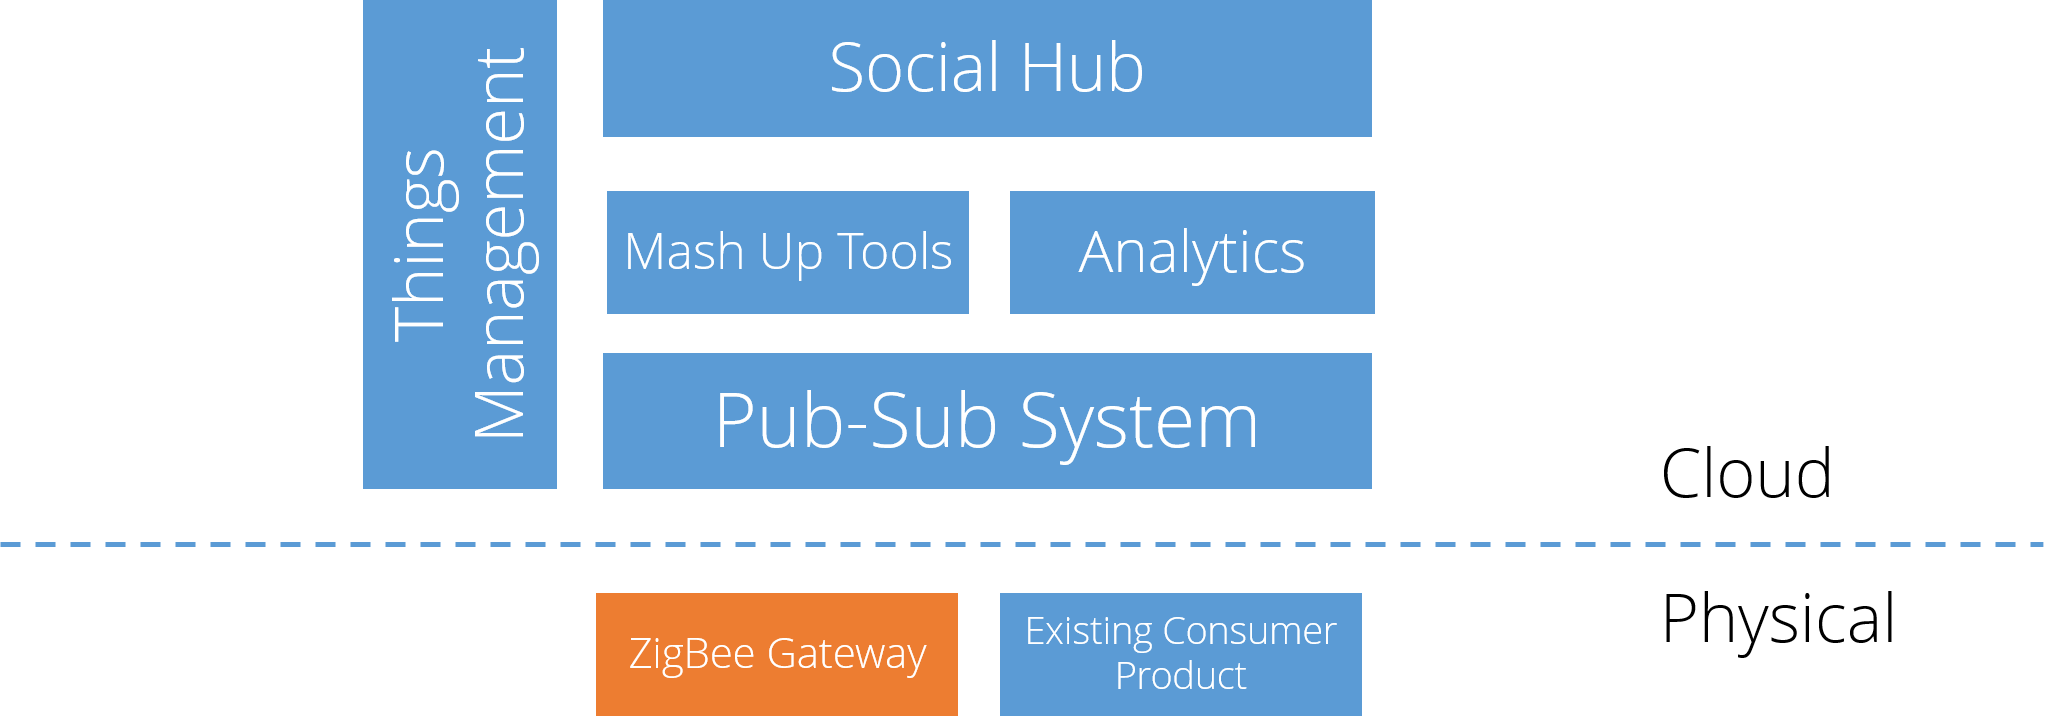
\includegraphics[width=.9\textwidth]{pics/rancangan-siot.PNG}
	\caption{Gambaran Umum \textit{Platform} \textit{social}~\IOT~berbasis media sosial}
	\label{fig:rancangan-siot}
\end{figure}

Sistem ini terdiri dari beberapa bagian yang saling berhubungan. Sebagian besar sistem ini berada di \textit{server} yang terhubung dengan jaringan internet. Penjelasan lebih detail mengenai bagian-bagian tersebut adalah sebagai berikut:
\begin{enumerate}
	\item \textit{Social Hub}
	
	Bagian ini merupakan abstraksi teratas dalam keseluruhan sistem. Bagian ini sekaligus menjadi \textit{user interface}, dimana penggunga \plat~nantinya akan mengakses sistem ini. Selain menjadi tempat pengguna mendaftar, bagian ini juga memiliki fungsi yang sangat penting, yaitu mengatur bagaimana mekanisme pembagian hak akses dan hak kontrol diantara seorang pengguna dengan pengguna lainnya. Sebagai contoh, pengguna dapat memilih apakah hak akses informasi mengenai sebuah perangkat yang dimilikinya akan dibagikan ke seluruh pengguna internet, hanya teman-temannya saja, atau hanya orang-orang tertentu saja.
	
	\item \textit{Mash Up Tools}
	
	\textit{Mash up tools} merupakan salah satu cara bagi pengguna \plat~untuk berinteraksi dengan suatu perangkat. Melalui \textit{mash up tools}, pengguna dapat melakukan otomasi terhadap sebuah perangkat jika memenuhi kondisi tertentu. Misalnya, seorang pengguna dapat mengatur agar lampu ruang keluarga yang dimilikinya akan otomatis menyala jika pengguna mendapat email dengan subjek tertentu.
	
	\item \textit{Analytics}
	
	Dengan banyaknya perangkat yang nantinya akan terhubung ke \plat~ini, akan sangat banyak pula data yang melewati sistem ini. Data-data tersebut jika dilihat secara terpisah mungkin tidak memiliki nilai yang berarti. Namun, jika data seperti ini terdapat dalam jumlah yang sangat banyak, kita mungkin bisa mendapatkan wawasan tentang suatu hal yang terkait dengan data tersebut. Oleh karena itu, diperlukan suatu bagian yang dapat mengolah data yang banyak ini sehingga dapat memberikan suatu informasi yang berarti. Inilah peran dari bagian \textit{analytics}.
	
	\item \textit{Pub-Sub System}
	
	Seperti yang telah disebutkan sebelumnya, seiring dengan semakin banyaknya pengguna yang terdaftar dan perangkat yang terhubung, akan semakin banyak pula data yang akan melewati sistem ini. Data-data ini harus dikirimkan dari satu perangkat ke setiap pengguna yang berhak menerimanya, dan juga dari pengguna ke setiap perangkat yang harus menerimanya. Oleh karena itu, diperlukan suatu mekanisme pengaturan pengiriman pesan, yang dapat mengirimkan setiap data tersebut ke tujuan yang sesuai dan tetap menjaga kualitas kinerja dari sistem. Hal terkait mekanisme pengiriman pesan inilah yang ditangani oleh \textit{pub-sub system}.
	
	\item \textit{Things Management}
	
	\textit{Things management} adalah bagian yang mengatur hubungan antara sistem ini dengan setiap perangkat yang terhubung. \textit{Things management} mengatur mulai dari proses pendaftaran perangkat, hingga penyimpanan informasi terkait perangkat. Things management ini juga yang mengatur bagaimana mekanisme komunikasi antara \plat~dengan perangkat. Perangkat yang terhubung dengan bagian ini terbagi menjadi dua macam. Yang pertama adalah perangkat yang sudah tersedia di pasaran saat ini. Untuk perangkat jenis ini, \textit{things management} akan menggunakan API perangkat terkait sebagai jalur komunikasi dengan perangkat tersebut. Dengan demikian, perangkat yang sudah dimiliki pengguna dapat langsung dihubungkan dengan \plat~ini. Jenis kedua adalah perangkat yang akan dikembangkan di masa depan. Untuk perangkat jenis ini, \textit{things management} akan menyediakan sebuah API yang dapat digunakan oleh pengembang perangkat cerdas, sehingga perangkat yang dikembangkannya dapat terhubung dengan \plat~ini.
	
	\item \textit{Gateway}
	
	Bagian yang terakhir adalah \textit{gateway}. Bagian ini berfungsi menghubungkan suatu perangkat dengan internet, khususnya \plat~ini. \textit{Gateway} inilah yang akan \saya~implementasikan dalam tugas akhir ini. Dalam sistem ini, \textit{gateway} berhubungan dengan \textit{things management} sebagai perangkat jenis kedua. Oleh karena itu, dalam melakukan implementasi \textit{gateway} ini \saya~akan mengacu pada API yang disediakan oleh \textit{things management}. Meskipun di masa mendatang diharapkan \textit{gateway} bisa menghubungkan berbagai jenis perangkat, namun untuk implementasi saat ini \saya~akan fokus pada perangkat lampu yang menggunakan teknologi ZigBee. Selain lampu, \textit{gateway} ini juga bisa mengontrol sebuah kumpulan lampu, atau biasa disebut sebagai \textit{group}. Karena atribut yang dimiliki oleh lampu dan \textit{group} sama, maka dalam tugas akhir ini sebuah \textit{group} akan diibaratkan sebagai sebuah lampu.
	
\end{enumerate}

\subsection{Gambaran Umum Perangkat \textit{Gateway}}
Dalam tugas akhir ini diimplementasikan sebuah perangkat \textit{gateway} yang menghubungkan jaringan lampu berbasis ZigBee dengan internet. Jaringan lampu ini secara spesifik akan dihubungkan dengan \textit{social}\iot~\plat~berbasis media sosial dengan deskripsi seperti yang telah dijelaskan sebelumnya. Pertama kali, lampu akan didaftarkan ke bagian \textit{things management} pada \plat~, kemudian setelah terdaftar, \textit{gateway} akan secara periodik mengirimkan informasi mengenai lampu ke \textit{pub-sub system} dan menerima perintah dari \textit{pub-sub system}. Gambar \ref{fig:rancangan-sistem} menunjukkan visualisasi hubungan perangkat \textit{gateway} dengan \plat~dan lampu.

\begin{figure}
	\centering
	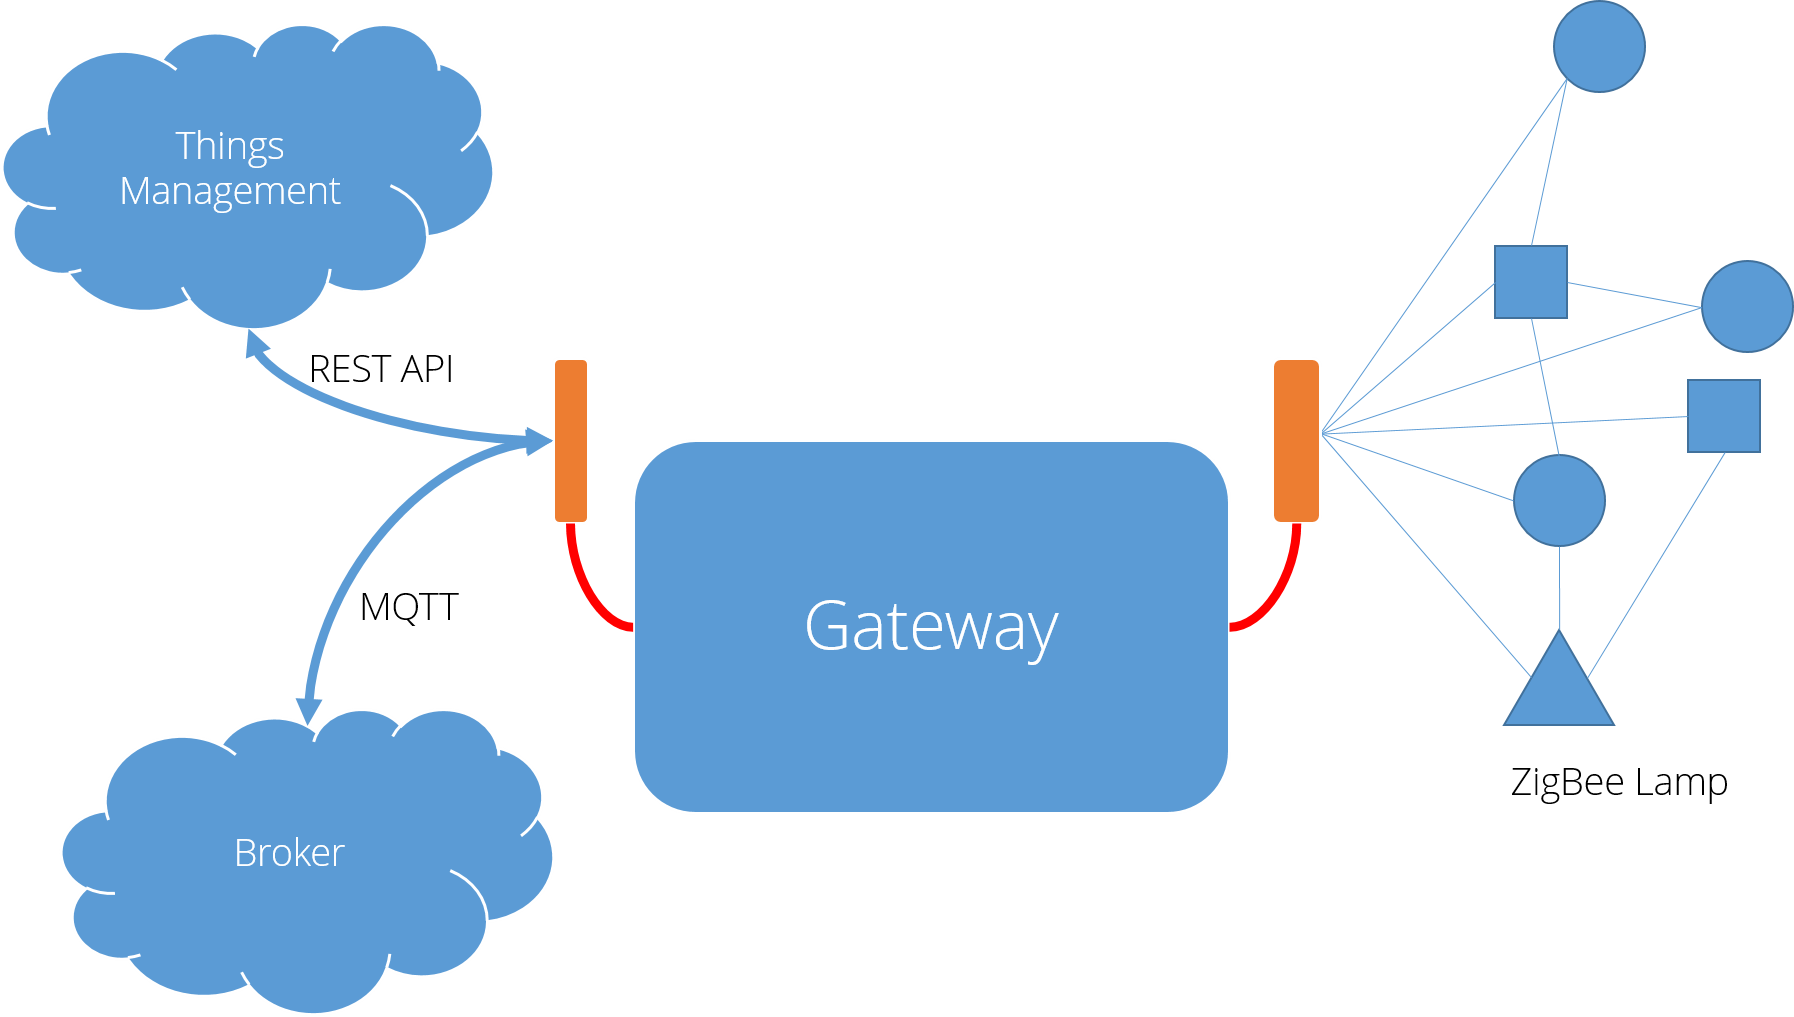
\includegraphics[width=.9\textwidth]{pics/rancangan-sistem.PNG}
	\caption{Gambaran Umum Sistem}
	\label{fig:rancangan-sistem}
\end{figure}

Sistem ini terdiri dari jaringan lampu ZigBee, sebuah perangkat \textit{gateway}, dan \textit{social}\iot~\plat~berbasis media sosial. Di dalam \plat~\iot~terdapat \textit{things management} yang bertugas sebagai portal manajemen perangkat, termasuk mendaftarkan dan menyimpan informasi terkait perangkat, dan sebuah \textit{pub-sub system} yang bertugas untuk menyampaikan data yang dikirimkan ke dan dari \textit{gateway}. \textit{Gateway} akan menarik informasi mengenai keadaan lampu melalui jaringan ZigBee, kemudian jika lampu belum didaftarkan ke \plat, maka pengguna dapat mendaftarkan lampu tersebut. Proses pendaftaran lampu ini menggunakan REST melalui API yang disediakan. Setelah didaftarkan, \textit{gateway} kemudian akan mengirimkan informasi mengenai lampu terkait secara periodik ke \plat. Informasi ini akan dikirimkan melalui protokol MQTT ke \textit{pub-sub system} yang terdapat pada \plat. Implementasi \textit{pub-sub system} pada \plat~menggunakan Mosquitto. Selain itu, \textit{gateway} juga dapat digunakan sebagai alat untuk mengontrol lampu-lampu yang terdapat dalam jaringan ZigBee.

Gambar \ref{fig:rancangan-gateway} menunjukkan visualisasi yang lebih mendetail pada sistem internal perangkat \textit{gateway}. Untuk bisa terhubung dengan jaringan ZigBee, dibutuhkan sebuah \textit{coordinator}. Pada tugas akhir ini, implementasi ZigBee \textit{coordinator} yang akan digunakan adalah implementasi yang dibuat oleh pihak Dresden Elektronik dengan nama deCONZ. deCONZ mengimplementasikan profile \textit{light link} yang disediakan oleh pihak ZigBee Alliance, sehingga dapat digunakan untuk menghubungkan lampu ZigBee yang menggunakan profil yang sama. Perangkat yang digunakan untuk terhubung ke lampu ZigBee adalah sebuah \textit{shield} Raspberry Pi bernama RaspBee yang juga dibuat oleh Dresden Elektronik dan dapat dihubungkan ke \textit{port} GPIO yang terdapat pada Raspberry Pi. Secara \textit{default}, deCONZ dapat berkomunikasi dengan RaspBee tanpa perlu dilakukan banyak konfigurasi.

\begin{figure}
	\centering
	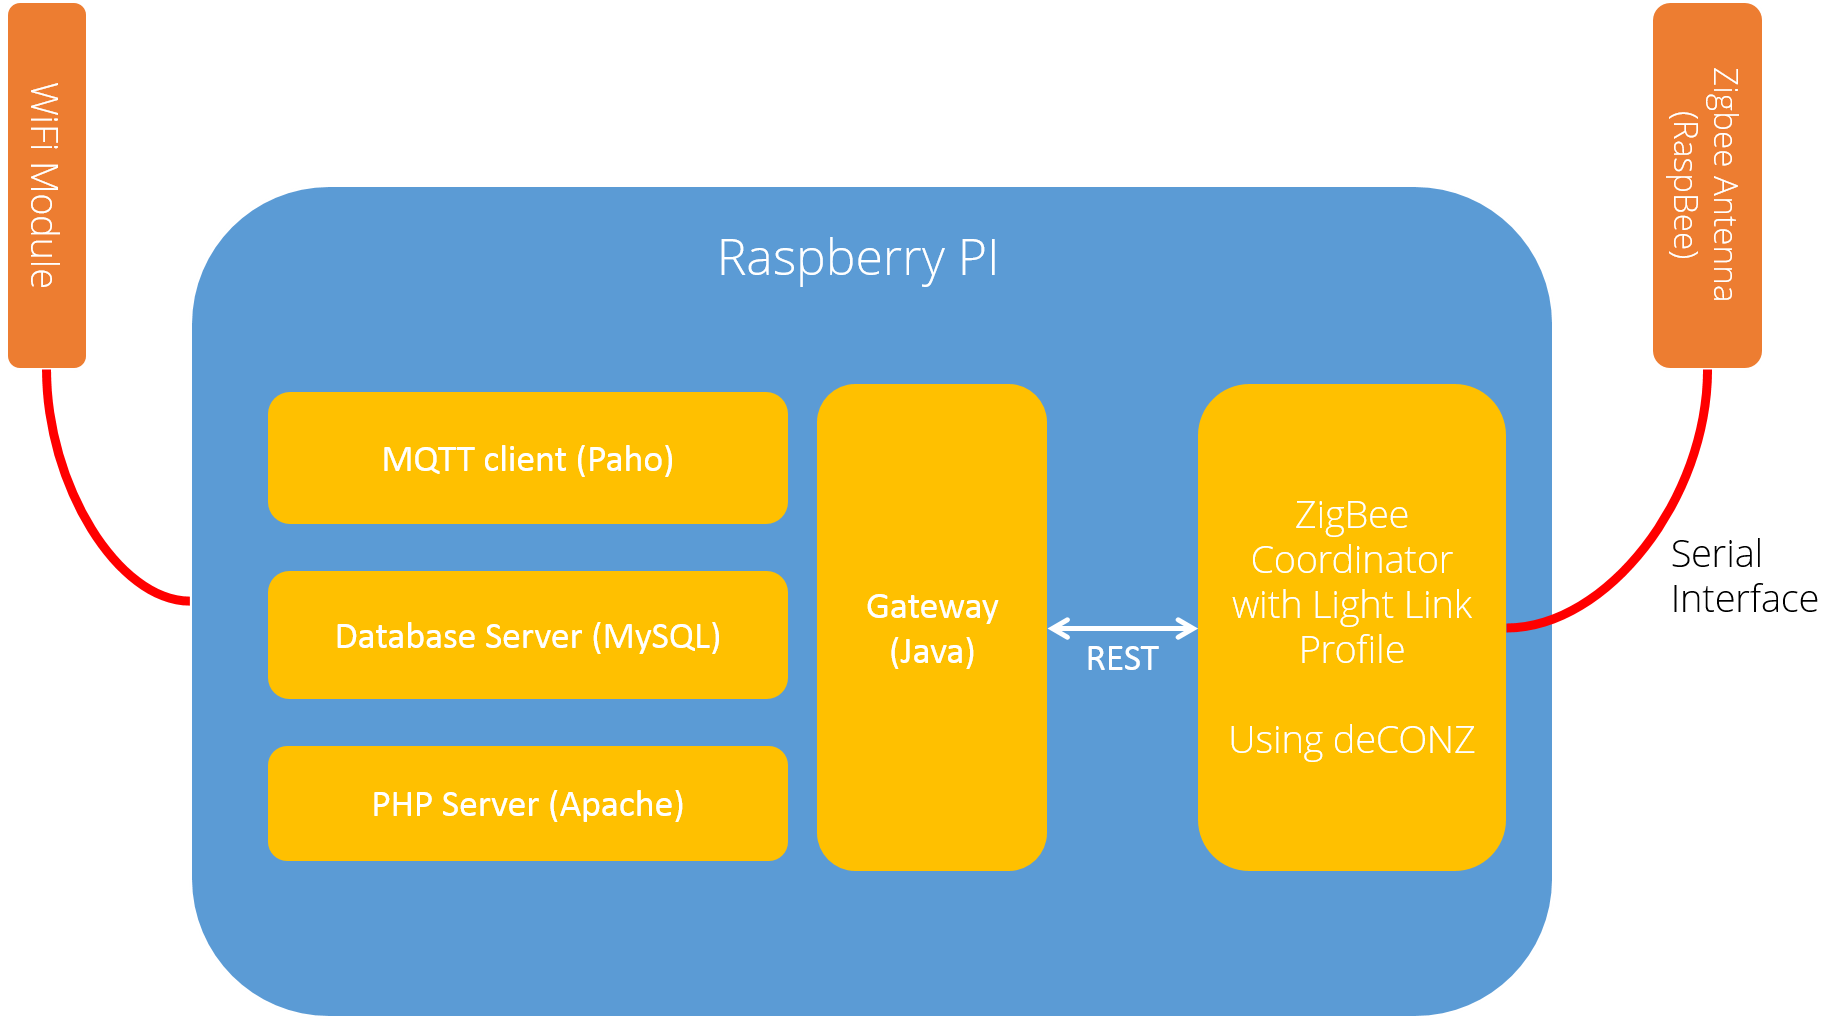
\includegraphics[width=.9\textwidth]{pics/rancangan-gateway.PNG}
	\caption{Gambaran Umum Gateway}
	\label{fig:rancangan-gateway}
\end{figure} 

\textit{Gateway} pada tugas akhir ini akan bertugas mengirimkan informasi mengenai lampu ZigBee yang terhubung secara berkala ke \plat~, dan juga menerima perintah yang datang dari \plat~untuk kemudian disampaikan ke lampu terkait. Implementasi \textit{gateway} dikerjakan menggunakan bahasa pemrograman Java. Ketika dijalankan, \textit{gateway} akan membuat sebuah MQTT \textit{client} yang diimplementasikan menggunakan \textit{library} Eclipse Paho. MQTT \textit{client} inilah yang akan digunakan untuk menerima perintah dari \plat~dan secara berkala mengirim informasi ke \plat. Perangkat ini juga akan menyediakan sebuah aplikasi web yang dapat digunakan untuk mengontrol dan mengelola lampu yang terhubung. Melalui aplikasi web ini, pengguna dapat mendaftarkan lampu yang dimilikinya ke \textit{things management} yang terdapat pada \plat. Informasi terkait hasil pendaftaran ini akan disimpan pada sebuah \textit{database server} dan akan digunakan selanjutnya oleh \textit{gateway} untuk menentukan beberapa hal, seperti \textit{id} lampu yang tersimpan di \textit{things management}, perintah apa saja yang akan diterima oleh \textit{gateway}, dan informasi apa saja yang akan dibagikan oleh \textit{gateway}.Pada perangkat ini juga akan dipasang sebuah modul WiFi yang dapat digunakan untuk menghubungkan perangkat \textit{wifi} ke internet dan untuk mengakses aplikasi web pada perangkat \textit{gateway}.

\section{Rancangan Implementasi \textit{Gateway}}
Pada subbab ini akan dijelaskan secara mendetail mengenai rancangan perangkat \textit{gateway} yang dibuat. Penjelasan pada subbab ini mencakup perangkat dan \textit{tools} yang digunakan, mekanisme pengiriman pesan beserta topik yang digunakan, dan rancangan cara penggunaan perangkat \textit{gateway}.

\subsection{Perangkat yang digunakan}
Perangkat yang akan digunakan pada pengerjaan tugas akhir ini adalah Raspberry Pi. Raspberry Pi adalah sebuah komputer berukuran kecil, yang dikembangkan oleh yayasan Raspberry Pi. Walaupun berukuran kecil, Raspberry Pi merupakan sebuah komputer yang dapat berfungsi penuh seperti komputer biasa. OS yang tersedia untuk Raspberry Pi cukup banyak dan dapat diunduh langsung dari situs resmi Raspberry Pi. Raspberry Pi dipilih untuk pengerjaan tugas akhir ini karena memiliki kemampuan yang cukup untuk menjalankan berbagai kebutuhan pada implementasi perangkat \textit{gateway} ini. Selain itu, Raspberry Pi memiliki harga yang cukup murah, hanya sekitar enam ratus ribu rupiah untuk tipe terbaru. 

Untuk bisa terhubung dengan sebuah jaringan ZigBee, diperlukan juga sebuah perangkat yang memiliki kemampuan untuk menangkap sinyal ZigBee dan terhubung dengan jaringan ZigBee. Perangkat ini juga harus bisa digunakan pada perangkat Raspberry Pi. Perangkat yang dipilih untuk implementasi pada tugas akhir ini adalah RaspBee, sebuah \textit{shield} untuk Raspberry Pi yang diproduksi oleh Dresden Elektronik. RaspBee dipilih untuk pengerjaan tugas akhir ini karena memiliki \textit{tools} yang dapat digunakan untuk menghubungkan jaringan ZigBee dengan mudah, dan \textit{tools} tersebut dapat dijalankan pada Raspberry Pi. 

\subsection{\textit{Tools} yang digunakan}
Implementasi perangkat \textit{gateway} pada tugas akhir ini menggunakan beberapa \textit{tools} yang sudah tersedia. \textit{Tools} yang digunakan adalah deCONZ, Mosquitto, dan Eclipse Paho.

\subsubsection{deCONZ}
deCONZ merupakan paket aplikasi yang dibuat dan disebarkan secara gratis oleh Dresden Elektronik. Aplikasi ini dapat digunakan untuk menghubungkan beberapa perangkat yang diproduksi oleh Dresden Elektronik dengan jaringan perangkat berbasis ZigBee. 

Terdapat tiga cara untuk menggunakan deCONZ. Yang pertama adalah dengan menggunakan aplikasi GUI yang termasuk dalam satu set aplikasi deCONZ. Untuk menggunakan aplikasi GUI ini, Raspberry Pi harus dihubungkan ke layar eksternal dan OS dalam Raspberry Pi harus menjalankan sebuah X server atau tampilan \textit{desktop}. deCONZ dalam mode GUI ini bisa terhubung dengan semua perangkat berbasis ZigBee. Gambar \ref{fig:deconz-gui} menunjukkan tampilan deCONZ ketika dijalankan dalam mode GUI

\begin{figure}
	\centering
	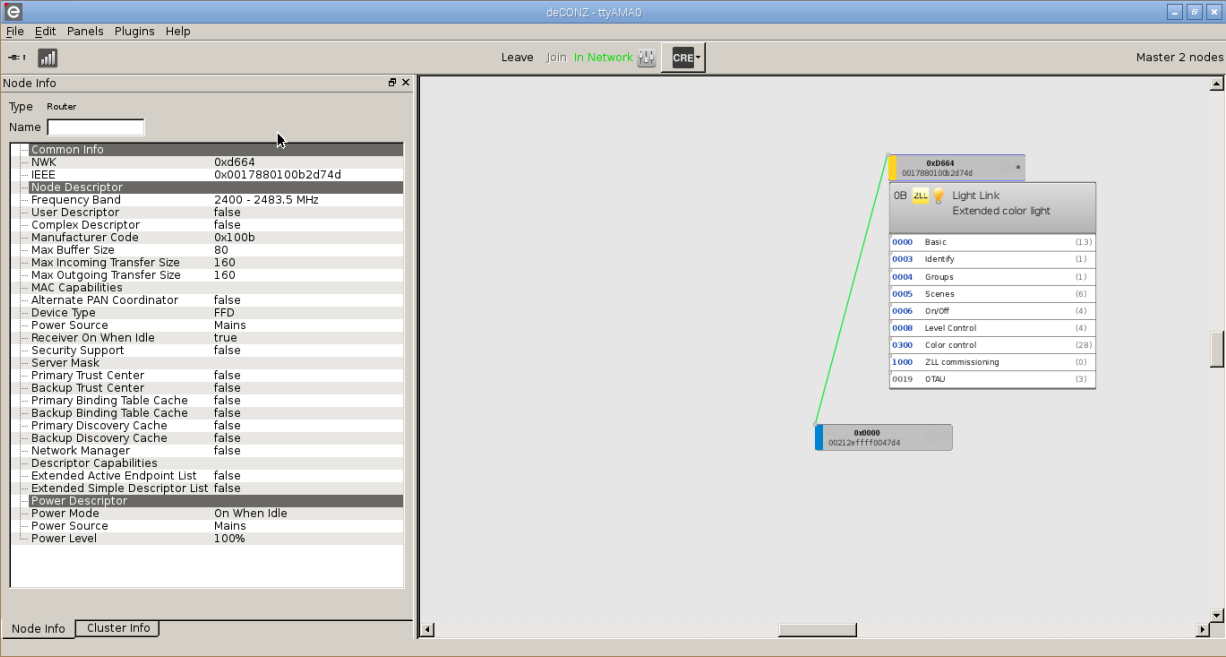
\includegraphics[width=.9\textwidth]{pics/deCONZ-gui.png}
	\caption{Tampilan Aplikasi deCONZ berbasis GUI}
	\label{fig:deconz-gui}
\end{figure}

Cara kedua adalah menggunakan aplikasi web yang juga sudah termasuk dalam set aplikasi deCONZ. Ketika dijalankan, aplikasi deCONZ akan sekaligus menjalankan sebuah \textit{webserver} dimana aplikasi web deCONZ dijalankan. Untuk mengakses aplikasi web ini, kita dapat menggunakan browser dari desktop di \rasp~, atau dari perangkat di luar \rasp~menggunakan koneksi jaringan seperti Ethernet atau WiFi. Jika mengakses dari luar \rasp~, maka kita perlu mengetahui alamat IP dari \rasp~ketika sedang digunakan. Aplikasi deCONZ yang berbasis web ini hanya dapat digunakan untuk mengontrol perangkat berbasis ZigBee yang menggunakan profil \textit{Light Link} atau \textit{Home Automation} dengan jenis lampu. Gambar \ref{fig:deconz-web} menunjukkan tampilan aplikasi deCONZ berbasis web.

\begin{figure}
	\centering
	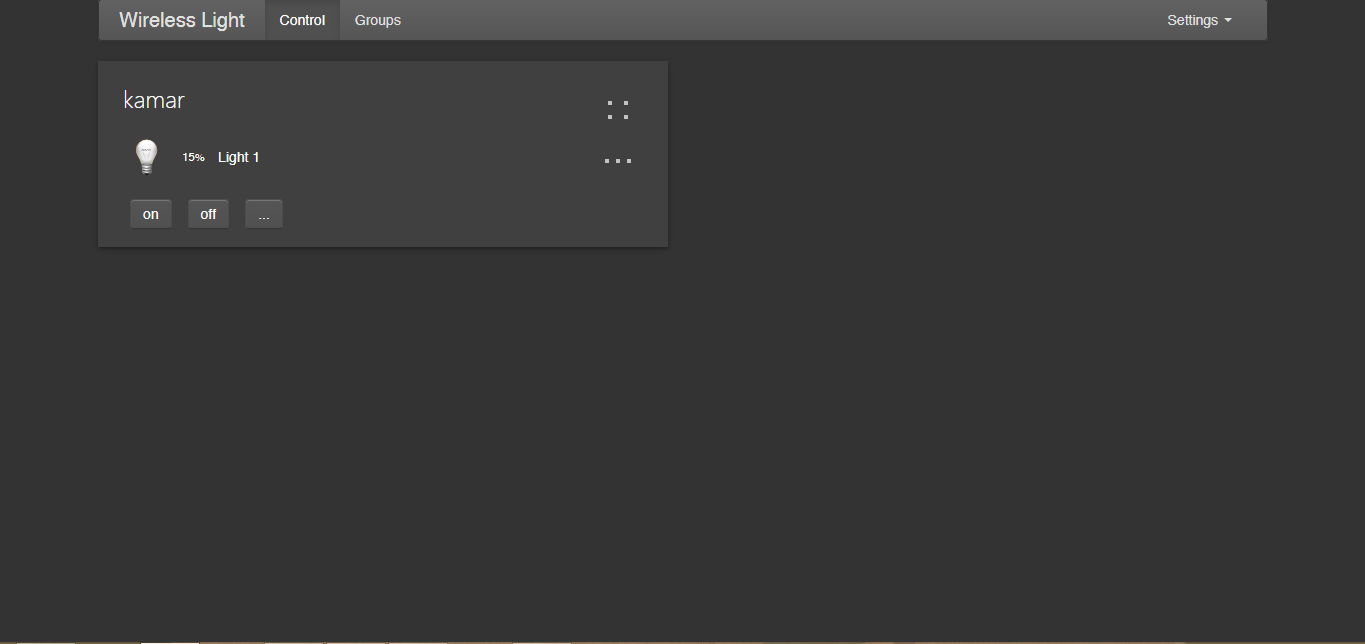
\includegraphics[width=.9\textwidth]{pics/deCONZ-web.png}
	\caption{Tampilan Aplikasi deCONZ berbasis web}
	\label{fig:deconz-web}
\end{figure}

Cara terakhir adalah menggunakan REST API. Sama seperti sebelumnya, ketika dijalankan deCONZ juga akan sekaligus menjalankan sebuah \textit{webserver}, yang juga menjadi tempat di mana REST API ini berjalan. Untuk bisa mengakses REST API ini, kita bisa menggunakan koneksi jaringan dari luar \rasp~atau mengaksesnya langsung dari dalam \rasp. Untuk implementasi \textit{gateway} pada tugas akhir ini, cara yang akan digunakan adalah melalui REST API.

\subsubsection{Mosquitto}
Mosquitto adalah sebuah broker \textit{open source} yang mengimplementasikan protokol MQTT versi 3.1 dan 3.1.1. Mosquitto dapat diunduh melalui situs resminya, dan tersedia untuk banyak \textit{platform}, mulai dari Windows, Mac, beberapa distro linux termasuk untuk Raspberry Pi, hingga iOS. Mosquitto juga sudah menyediakan \textit{client} untuk melakukan proses \textit{publishing} dan \textit{subscribing} melalui \textit{command line}. Pada tugas akhir ini, Mosquitto digunakan sebagai broker yang dipasang pada \textit{pub-sub system} di \plat~\iot~yang dikembangkan oleh \saya~dan teman-teman \saya.

\subsubsection{Eclipse Paho}
Paho merupakan sebuah implementasi \textit{client MQTT} yang dikembangkan oleh Eclipse dan bersifat \textit{open source}. Implementasi ini dibungkus menjadi suatu \textit{library} yang dapat digunakan di beberapa bahasa dan dapat diunduh melalui situs resminya. Beberapa bahasa yang didukung oleh \textit{library} Eclipse Paho saat ini adalah Java, Phyton, Javascript, C/C++, dan .Net. Pada tugas akhir ini, \textit{library} yang digunakan adalah Eclipse Paho untuk bahasa Java, dan akan digunakan sebagai \textit{client} yang akan berjalan pada perangkat \textit{gateway}.

\subsection{Rancangan Mekanisme Pengiriman Pesan}
Ketika dijalankan, \textit{gateway} akan membuat dua buah \textit{client} MQTT menggunakan Eclipse paho. \textit{Client} yang pertama akan berperan sebagai \textit{publisher} dan \textit{client} yang kedua sebagai \textit{subscriber}. Setiap sepuluh detik, \textit{gateway} akan mengambil informasi mengenai lampu yang terhubung ke \textit{coordinator}, dan mengirimkan informasi tersebut ke \textit{pub-sub system} yang terdapat pada \plat~melalui mekanisme \textit{publishing}. \textit{Subscriber} pada \textit{gateway} akan selalu menunggu pesan yang datang dari \textit{pub-sub system}. Jika pesan yang diterima berupa perintah, maka perintah tersebut akan diubah menjadi perintah REST yang akan dikirimkan ke deCONZ. Visualisasi mekanisme ini ditampilkan pada gambar \ref{fig:rancanan-pengiriman-pesan}.

\begin{figure}
	\centering
	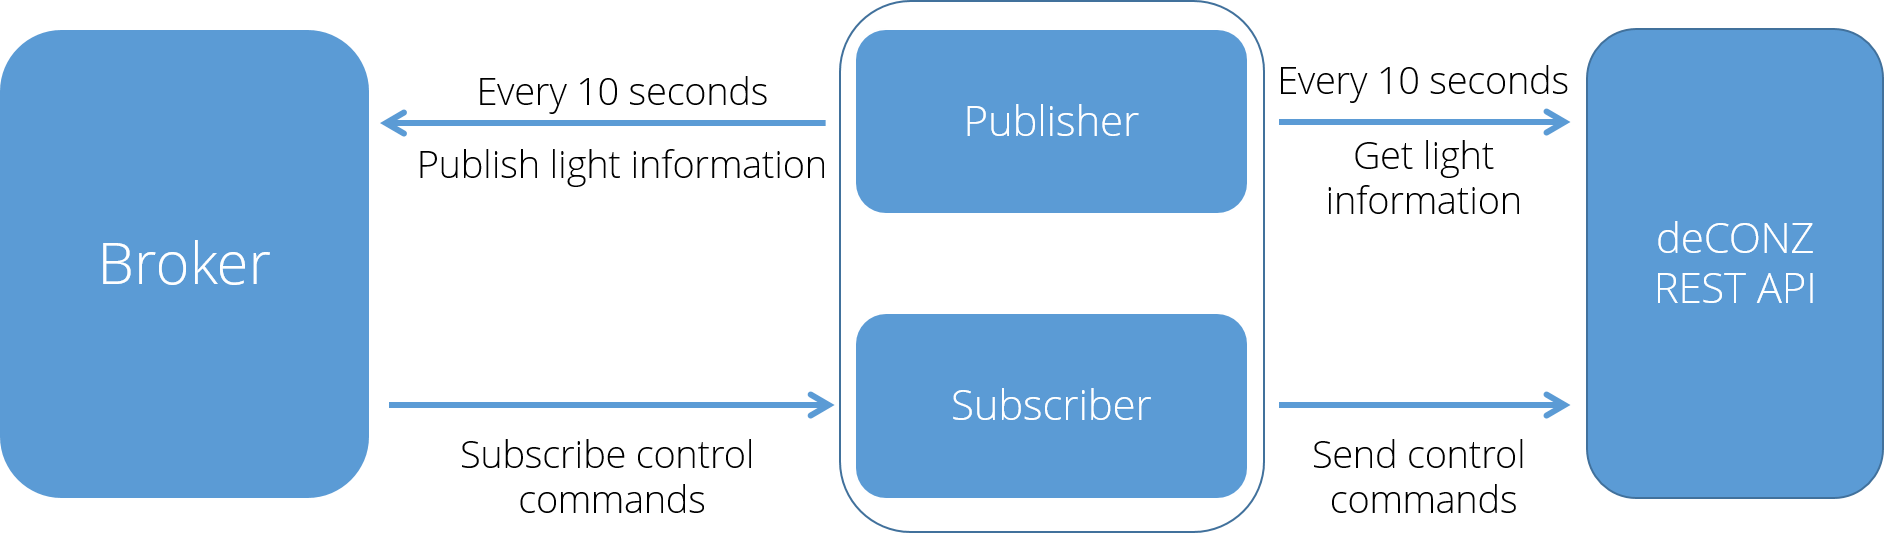
\includegraphics[width=.9\textwidth]{pics/rancangan-pengiriman-pesan.png}
	\caption{Rancangan Mekanisme Pengiriman Pesan}
	\label{fig:rancanan-pengiriman-pesan}
\end{figure}

\subsection{Rancangan Topik}
Topik yang digunakan pada \plat~\iot~ini dibuat agar menjadi sebuah topik yang bersifat \textit{generic}, sehingga topik ini tetap bisa digunakan apapun jenis perangkat yang nantinya akan terhubung. Pertama, untuk menandai bahwa topik ini digunakan untuk \plat~yang \saya~dan teman-teman \saya~buat, topik ini diawali dengan \texttt{sot/}. Selanjutnya, karena \plat~yang digunakan akan mengelola dua jenis perangkat yang berbeda (lihat subbab 3.1 bagian \textit{things management}), maka selanjutnya ditambahkan \texttt{/d} untuk menandakan perangkat jenis pertama atau \texttt{/g} untuk menandakan atau perangkat jenis kedua. Karena perangkat \textit{gateway} merupakan perangkat jenis kedua, maka akan digunakan \texttt{/g} dalam topik pada tugas akhir ini. Topik ini juga harus bisa mengatasi penggunaan oleh banyak pengguna, sehingga harus ada informasi mengenai identitas pengguna di dalam topik. Oleh karena itu, ditambahkan \texttt{/[idUser]} ke dalam topik.

Selanjutnya, \plat~juga memiliki kebutuhan untuk mengetahui jenis perangkat dalam suatu topik, maka ditambahkan \texttt{/[kategori]} ke dalam topik. Karena dalam tugas akhir ini perangkat yang digunakan hanya lampu, maka kategori yang digunakan adalah \texttt{ledlight}. Kemudian, \textit{gateway} juga perlu mengetahui informasi tentang perangkat mana yang menjadi tujuan atau pengirim informasi di dalam topik, maka ditambahkan \texttt{[idPerangkat]} ke dalam topik. Terakhir, terdapat dua buah operasi terkait sebuah atribut dalam suatu perangkat yaitu untuk mengontrol, atau memberikan informasi mengenai perangkat. Oleh karena itu, ditambahkan \texttt{/[atribut]/(acc atau ctl)} pada bagian akhir dari topik. \texttt{acc} menandakan bahwa topik tersebut mengirimkan pesan yang berisi informasi mengenai perangkat ke \plat~, sedangkan \texttt{ctl} menandakan bahwa pesan yang dikirimkan berisi perintah yang ditujukan ke perangkat. Jika digabungkan, topik yang akan digunakan pada tugas akhir ini menjadi \texttt{sot/g/[idUser]/ledlight/[idPerangkat]/[atribut]/(acc atau ctl)}.

\subsection{Rancangan Translasi Pesan MQTT Menjadi Perintah REST}
Ketika \textit{gateway} menerima pesan untuk mengontrol suatu lampu, \textit{gateway} perlu menerjemahkan pesan tersebut menjadi sebuah perintah REST yang kemudian disampaikan ke deCONZ. Informasi yang dibutuhkan untuk mengontrol lampu atau \textit{group} terdapat di dalam topik dan juga di dalam pesan yang dikirimkan. Selain itu, terdapat perbedaan id yang digunakan dalam \textit{things management} di \plat~dan id yang digunakan deCONZ untuk menghubungi lampu, sehingga \textit{gateway} juga perlu menyimpan informasi mengenai kedua id pada masing-masing lampu. Dalam bagian ini, id lampu yang disimpan pada \textit{things managemement} akan dituliskan dengan \texttt{idPerangkat}, dan id lampu yang digunakan oleh deCONZ akan dituliskan dengan \texttt{idLokal}. Selain itu, untuk bisa mengakses API REST yang disediakan oleh deCONZ, diperlukan suatu kunci API. Pada tugas akhir ini, kunci yang digunakan adalah \texttt{LUQMANGWTA}. Berikut merupakan contoh pesan-pesan yang akan diterima oleh \textit{gateway} dan akan disampaikan ke deCONZ.

\begin{enumerate}
	\item Menghidupkan lampu
	
	Berikut merupakan contoh topik dan pesan yang dikirimkan untuk menghidupkan lampu.
	
	\begin{table}
		\centering
		\caption{Contoh pesan dan topik untuk menghidupkan lampu}
		\label{tab:nyalainLampu}
		\begin{tabular}{|l |p{11cm} |}
			\hline
			\textbf{Topik} & \texttt{sot/g/[idUser]/ledlight/[idPerangkat]/on/ctl} \\
			\hline
			\textbf{Isi pesan} & \texttt{true} \\
			\hline
			\textbf{Perintah REST }& \texttt{PUT http://localhost:8080/api/LUQMANGWTA/ lights/[idLokal]/state}\\
			\hline
			\textbf{Data yang dikirimkan} & \texttt{\{"on":true\}} \\
			\hline
			\textbf{Respon deCONZ} & \texttt{[\{"success":\{"/lights/[idLokal]/state/on":true\}\}]} \\
			\hline
		\end{tabular}
	\end{table}
	
	
	\item Mematikan Lampu
	
	Berikut merupakan contoh topik dan pesan yang dikirimkan untuk mematikan lampu.
	
	\begin{table}
		\centering
		\caption{Contoh pesan dan topik untuk mematikan lampu}
		\label{tab:matiinLampu}
		\begin{tabular}{| l | p{11cm} |}
			\hline
			\textbf{Topik} & \texttt{sot/g/[idUser]/ledlight/[idPerangkat]/on/ctl} \\
			\hline
			\textbf{Isi pesan} & \texttt{false} \\
			\hline
			\textbf{Perintah REST} & \texttt{PUT http://localhost:8080/api/LUQMANGWTA/ lights/[idLokal]/state} \\
			\hline
			\textbf{Data yang dikirimkan} & \texttt{\{"on":false\}} \\
			\hline
			\textbf{Respon deCONZ} & \texttt{[\{"success":\{"/lights/[idLokal]/state/on":false\}\}]} \\
			\hline
		\end{tabular}
	\end{table}
	
	\item Mengubah Tingkat Kecerahan Lampu (\textit{Brightness})
	
	Berikut merupakan contoh topik dan pesan yang dikirimkan untuk mengubah tingkat kecerahan lampu.
	
	\begin{table}
		\centering
		\caption{Contoh pesan dan topik untuk mengubah tingkat kecerahan lampu}
		\label{tab:brightnessLampu}
		\begin{tabular}{| l | p{11cm} |}
			\hline
			\textbf{Topik} & \texttt{sot/g/[idUser]/ledlight/[idPerangkat]/bri/ctl} \\
			\hline
			\textbf{Isi pesan} & \texttt{100} \\
			\hline
			\textbf{Perintah REST} & \texttt{PUT http://localhost:8080/api/LUQMANGWTA/ lights/[idLokal]/state} \\
			\hline
			\textbf{Data yang dikirimkan} & \texttt{\{"bri":100\}} \\
			\hline
			\textbf{Respon deCONZ} & \texttt{[\{"success":\{"/lights/[idLokal]/state/bri":100\}\}]} \\
			\hline
		\end{tabular}
	\end{table}
	
	\item Mengubah Warna Lampu (\textit{Hue})
	
	Berikut merupakan contoh topik dan pesan yang dikirimkan untuk mengubah warna lampu.
	
	\begin{table}
		\centering
		\caption{Contoh pesan dan topik untuk mengubah warna lampu}
		\label{tab:hueLampu}
		\begin{tabular}{| l | p{11cm} |}
			\hline
			\textbf{Topik} & \texttt{sot/g/[idUser]/ledlight/[idPerangkat]/hue/ctl} \\
			\hline
			\textbf{Isi pesan} & \texttt{45000} \\
			\hline
			\textbf{Perintah REST} & \texttt{PUT http://localhost:8080/api/LUQMANGWTA/ lights/[idLokal]/state} \\
			\hline
			\textbf{Data yang dikirimkan} & \texttt{\{"hue":45000\}} \\
			\hline
			\textbf{Respon deCONZ} & \texttt{[\{"success":\{"/lights/[idLokal]/state/hue":45000\}\}]} \\
			\hline
		\end{tabular}
	\end{table}
	
	\item Mengubah Tingkat Kejenuhan Lampu (\textit{Saturation})
	
	Berikut merupakan contoh topik dan pesan yang dikirimkan untuk mengubah warna lampu.
	
	\begin{table}
		\centering
		\caption{Contoh pesan dan topik untuk mengubah tingkat kejenuhan lampu}
		\label{tab:satLampu}
		\begin{tabular}{| l | p{11cm} |}
			\hline
			\textbf{Topik} & \texttt{sot/g/[idUser]/ledlight/[idPerangkat]/sat/ctl} \\
			\hline
			\textbf{Isi pesan} & \texttt{150} \\
			\hline
			\textbf{Perintah REST} & \texttt{PUT http://localhost:8080/api/LUQMANGWTA/ lights/[idLokal]/state} \\
			\hline
			\textbf{Data yang dikirimkan} & \texttt{\{"sat":246\}} \\
			\hline
			\textbf{Respon deCONZ} & \texttt{[\{"success":\{"/lights/[idLokal]/state/sat":246\}\}]} \\
			\hline
		\end{tabular}
	\end{table}
	
	\item Menghidupkan lampu di dalam suatu \textit{group}
	
	Berikut merupakan contoh topik dan pesan yang dikirimkan untuk menghidupkan lampu di dalam suatu \textit{group}.
	
	\begin{table}
		\centering
		\caption{Contoh pesan dan topik untuk menghidupkan lampu di dalam suatu \textit{group}}
		\label{tab:nyalainLampuInGroup}
		\begin{tabular}{|l |p{11cm} |}
			\hline
			\textbf{Topik} & \texttt{sot/g/[idUser]/ledlight/[idPerangkat]/on/ctl} \\
			\hline
			\textbf{Isi pesan} & \texttt{true} \\
			\hline
			\textbf{Perintah REST }& \texttt{PUT http://localhost:8080/api/LUQMANGWTA/ groups/[idLokal]/action}\\
			\hline
			\textbf{Data yang dikirimkan} & \texttt{\{"on":true\}} \\
			\hline
			\textbf{Respon deCONZ} & \texttt{[\{"success":\{"/groups/[idLokal]/action/on":true\}\}]} \\
			\hline
		\end{tabular}
	\end{table}
	
	
	\item Mematikan Lampu di dalam suatu \textit{group}
	
	Berikut merupakan contoh topik dan pesan yang dikirimkan untuk mematikan lampu di dalam suatu \textit{group}.
	
	\begin{table}
		\centering
		\caption{Contoh pesan dan topik untuk mematikan lampu di dalam suatu \textit{group}}
		\label{tab:matiinLampuInGroup}
		\begin{tabular}{| l | p{11cm} |}
			\hline
			\textbf{Topik} & \texttt{sot/g/[idUser]/ledlight/[idPerangkat]/on/ctl} \\
			\hline
			\textbf{Isi pesan} & \texttt{false} \\
			\hline
			\textbf{Perintah REST} & \texttt{PUT http://localhost:8080/api/LUQMANGWTA/ groups/[idLokal]/action} \\
			\hline
			\textbf{Data yang dikirimkan} & \texttt{\{"on":false\}} \\
			\hline
			\textbf{Respon deCONZ} & \texttt{[\{"success":\{"/groups/[idLokal]/action/on":false\}\}]} \\
			\hline
		\end{tabular}
	\end{table}
	
	\item Mengubah Tingkat Kecerahan Lampu (\textit{Brightness}) di dalam suatu \textit{group}
	
	Berikut merupakan contoh topik dan pesan yang dikirimkan untuk mengubah tingkat kecerahan lampu di dalam suatu \textit{group}.
	
	\begin{table}
		\centering
		\caption{Contoh pesan dan topik untuk mengubah tingkat kecerahan lampu di dalam suatu \textit{group}}
		\label{tab:brightnessLampuInGroup}
		\begin{tabular}{| l | p{11cm} |}
			\hline
			\textbf{Topik} & \texttt{sot/g/[idUser]/ledlight/[idPerangkat]/bri/ctl} \\
			\hline
			\textbf{Isi pesan} & \texttt{100} \\
			\hline
			\textbf{Perintah REST} & \texttt{PUT http://localhost:8080/api/LUQMANGWTA/ groups/[idLokal]/action} \\
			\hline
			\textbf{Data yang dikirimkan} & \texttt{\{"bri":100\}} \\
			\hline
			\textbf{Respon deCONZ} & \texttt{[\{"success":\{"/groups/[idLokal]/action/bri":100\}\}]} \\
			\hline
		\end{tabular}
	\end{table}
	
	\item Mengubah Warna Lampu (\textit{Hue}) di dalam suatu \textit{group}
	
	Berikut merupakan contoh topik dan pesan yang dikirimkan untuk mengubah warna lampu di dalam suatu \textit{group}.
	
	\begin{table}
		\centering
		\caption{Contoh pesan dan topik untuk mengubah warna lampu di dalam suatu \textit{group}}
		\label{tab:hueLampuInGroup}
		\begin{tabular}{| l | p{11cm} |}
			\hline
			\textbf{Topik} & \texttt{sot/g/[idUser]/ledlight/[idPerangkat]/hue/ctl} \\
			\hline
			\textbf{Isi pesan} & \texttt{45000} \\
			\hline
			\textbf{Perintah REST} & \texttt{PUT http://localhost:8080/api/LUQMANGWTA/ groups/[idLokal]/action} \\
			\hline
			\textbf{Data yang dikirimkan} & \texttt{\{"hue":45000\}} \\
			\hline
			\textbf{Respon deCONZ} & \texttt{[\{"success":\{"/groups/[idLokal]/action/hue":45000\}\}]} \\
			\hline
		\end{tabular}
	\end{table}
	
	\item Mengubah Tingkat Kejenuhan Lampu (\textit{Saturation}) di dalam suatu \textit{group}
	
	Berikut merupakan contoh topik dan pesan yang dikirimkan untuk mengubah warna lampu di dalam suatu \textit{group}.
	
	\begin{table}
		\centering
		\caption{Contoh pesan dan topik untuk mengubah tingkat kejenuhan lampu di dalam suatu \textit{group}}
		\label{tab:satLampuInGroup}
		\begin{tabular}{| l | p{11cm} |}
			\hline
			\textbf{Topik} & \texttt{sot/g/[idUser]/ledlight/[idPerangkat]/sat/ctl} \\
			\hline
			\textbf{Isi pesan} & \texttt{45000} \\
			\hline
			\textbf{Perintah REST} & \texttt{PUT http://localhost:8080/api/LUQMANGWTA/ groups/[idLokal]/action} \\
			\hline
			\textbf{Data yang dikirimkan} & \texttt{\{"sat":246\}} \\
			\hline
			\textbf{Respon deCONZ} & \texttt{[\{"success":\{"/groups/[idLokal]/action/sat":246\}\}]} \\
			\hline
		\end{tabular}
	\end{table}
	
\end{enumerate}

\subsection{Rancangan Mekanisme Penggunaan Oleh Pengguna}
Perangkat \textit{gateway} yang dibuat dalam tugas akhir ini ditujukan agar tetap bisa digunakan tanpa harus terhubung ke \plat~yang dikerjakan oleh \saya~dan teman-teman \saya. Oleh karena itu, dibutuhkan suatu cara untuk berinteraksi dengan pengguna yang tidak terlalu rumit. Selain itu, diperlukan juga cara mendaftarkan perangkat yang terhubung ke perangkat \textit{gateway} ke \textit{things management} pada \plat.

\subsubsection{Cara Pengguna Terhubung ke Perangkat \textit{Gateway}}
Ketika perangkat \textit{gateway} dinyalakan, perangkat \textit{gateway} akan berperan sebagai WiFi \textit{access point}. Pengguna kemudian dapat menggunakan komputer atau \textit{smartphone} yang dimilikinya untuk terhubung ke \textit{access point} yang dibuat oleh perangkat \textit{gateway}. Ketika pengguna terhubung ke perangkat \textit{gateway}, pengguna dapat membuka alamat \code{192.168.42.1/ta} menggunakan \textit{browser} yang dimiliki pengguna. Pada halaman itu, pengguna kemudian dapat memilih menu 'Pilih Access Point', dan pengguna akan diarahkan ke halaman yang menampilkan seluruh \textit{access point} yang berada dalam jangkauan perangkat \textit{gateway}. Pengguna kemudian dapat memilih \textit{access point} yang memiliki koneksi internet dan menghubungkan perangkat \textit{gateway} ke \textit{access point tersebut}. Pengguna kemudian akan diminta untuk menghubungkan \textit{smartphone} atau komputer yang digunakannya untuk dihubungkan ke \textit{access point} yang sama. Halaman tersebut juga akan memberikan sebuah tautan beserta alamat yang perlu dibuka untuk bisa kembali mengakses halaman aplikasi web perangkat \textit{gateway}.

\subsubsection{Cara Melakukan \textit{Log In} Melalui Perangkat \textit{Gateway}}
Untuk bisa mendaftarkan lampu atau \textit{group} yang terhubung ke perangkat \textit{gateway} ke \plat~, pengguna perlu melakukan \textit{log in} terlebih dahulu. Untuk melakukan \textit{log in}, pengguna harus sudah mendaftar terlebih dahulu di \plat. Setelah mendaftar, pengguna cukup melakukan klik pada tombol \textit{log in}, dan kemudian memasukkan \textit{email} yang sudah didaftarkan di \plat. Perangkat \textit{gateway} kemudian akan mendapatkan id pengguna dari \plat~, yang kemudian akan disimpan di dalam \textit{database} lokal untuk keperluan lain, seperti mendaftarkan lampu.

\subsubsection{Cara Mendaftarkan Lampu atau \textit{Group} ke \textit{Platform}}
Ketika membuka halaman web yang terdapat pada perangkat \textit{gateway}, pengguna dapat melihat daftar lampu yang terhubung. Pengguna kemudian dapat memilih opsi untuk mendaftarkan suatu lampu ke \plat. Ketika opsi tersebut dipilih, pengguna akan diminta untuk memilih atribut apa saja yang akan dibagikan ke \plat, dan atribut apa saja yang diperbolehkan untuk dikontrol dari \plat. Setelah didaftarkan, lampu tersebut akan mendapatkan sebuah id dari \textit{things management} pada platform. Id ini kemudian akan disimpan secara otomatis di dalam \textit{database} lokal di perangkat \textit{gateway}.

\section{Rancangan Pengujian}

Untuk memastikan perangkat yang dibuat berjalan dengan baik, perlu dilakukan suatu pengujian. Pengujian akan dilakukan dengan cara mencoba perangkat untuk menjalankan suatu kasus uji. Berikut adalah kasus uji yang akan diujikan pada perangkat yang dibuat:
\begin{enumerate}
	\item Kasus Uji 1: Menjadi \textit{access point}.
	\item Kasus Uji 2: Menghubungkan perangkat \textit{gateway} ke \textit{access point} lain.
	\item Kasus Uji 3: Menyalakan lampu melalui halaman web pada perangkat \textit{gateway}.
	\item Kasus Uji 4: Mematikan lampu melalui halaman web pada perangkat \textit{gateway}.
	\item Kasus Uji 5: Mengubah tingkat kecerahan lampu melalui halaman web pada perangkat \textit{gateway}.
	\item Kasus Uji 6: Mengubah warna lampu melalui halaman web pada perangkat \textit{gateway}.
	\item Kasus Uji 7: Mengubah tingkat kejenuhan lampu melalui halaman web pada perangkat \textit{gateway}.
	\item Kasus Uji 8: Membuat sebuah \textit{group} melalui halaman web pada perangkat \textit{gateway}.
	\item Kasus Uji 9: Menyalakan lampu dalam suatu \textit{group} melalui halaman web pada perangkat \textit{gateway}.
	\item Kasus Uji 10: Mematikan lampu dalam suatu \textit{group} melalui halaman web pada perangkat \textit{gateway}.
	\item Kasus Uji 11: Mengubah tingkat kecerahan lampu dalam suatu \textit{group} melalui halaman web pada perangkat \textit{gateway}.
	\item Kasus Uji 12: Mengubah warna lampu dalam suatu \textit{group} melalui halaman web pada perangkat \textit{gateway}.
	\item Kasus Uji 13: Mengubah tingkat kejenuhan lampu dalam suatu \textit{group} melalui halaman web pada perangkat \textit{gateway}.
	\item Kasus Uji 14: Mendaftarkan lampu ke \plat~melalui halaman web pada perangkat \textit{gateway}.
	\item Kasus Uji 15: Mendaftarkan \textit{group} ke \plat~melalui halaman web pada perangkat \textit{gateway}.
	\item Kasus Uji 16: Mengirimkan informasi mengenai atribut yang didaftarkan secara berkala ke \textit{pub-sub system}.
	\item Kasus Uji 17: Menyalakan lampu melalui pesan yang dikirimkan dari \textit{pub-sub system}.
	\item Kasus Uji 18: Mematikan lampu melalui pesan yang dikirimkan dari \textit{pub-sub system}.
	\item Kasus Uji 19: Mengubah tingkat kecerahan lampu melalui pesan yang dikirimkan dari \textit{pub-sub system}.
	\item Kasus Uji 20: Mengubah warna lampu melalui pesan yang dikirimkan dari \textit{pub-sub system}.
	\item Kasus Uji 21: Mengubah tingkat kejenuhan lampu melalui pesan yang dikirimkan dari \textit{pub-sub system}.
	\item Kasus Uji 22: Menyalakan lampu dalam suatu \textit{group} melalui pesan yang dikirimkan dari \textit{pub-sub system}.
	\item Kasus Uji 23: Mematikan lampu dalam suatu \textit{group} melalui pesan yang dikirimkan dari \textit{pub-sub system}.
	\item Kasus Uji 24: Mengubah tingkat kecerahan lampu dalam suatu \textit{group} melalui pesan yang dikirimkan dari \textit{pub-sub system}.
	\item Kasus Uji 25: Mengubah warna lampu dalam suatu \textit{group} melalui pesan yang dikirimkan dari \textit{pub-sub system}.
	\item Kasus Uji 26: Mengubah tingkat kejenuhan lampu dalam suatu \textit{group} melalui pesan yang dikirimkan dari \textit{pub-sub system}.	
\end{enumerate}

